%--------------------------------------------------------------
% thesis.tex 
%--------------------------------------------------------------
% Corso di Laurea in Informatica 
% http://if.dsi.unifi.it/
% @Facolt\`a di Scienze Matematiche, Fisiche e Naturali
% @Universit\`a degli Studi di Firenze
%--------------------------------------------------------------
% - template for the main file of Informatica@Unifi Thesis 
% - based on Classic Thesis Style Copyright (C) 2008 
%   Andr\'e Miede http://www.miede.de   
%--------------------------------------------------------------
\documentclass[twoside,openright,titlepage,fleqn,
	headinclude,11pt,a4paper,BCOR5mm,footinclude,draft
	]{scrbook}
%--------------------------------------------------------------
\newcommand{\myTitle}{Model checking come supporto per le scelte di sistemi adattivi\xspace}
% use the right myDegree option
\newcommand{\myDegree}{Corso di Laurea Magistrale in Informatica\xspace}
%\newcommand{\myDegree}{
	%Corso di Laurea Specialistica in Scienze e Tecnologie 
	%dell'Informazione\xspace}
\newcommand{\myName}{Marco Tinacci\xspace}
\newcommand{\myProf}{Rocco De Nicola\xspace}
\newcommand{\myOtherProf}{Michele Loreti\xspace}
%\newcommand{\mySupervisor}{Nome Cognome\xspace}
\newcommand{\myFaculty}{
	Facolt\`a di Scienze Matematiche, Fisiche e Naturali\xspace}
\newcommand{\myDepartment}{
	Dipartimento di Sistemi e Informatica\xspace}
\newcommand{\myUni}{\protect{
	Universit\`a degli Studi di Firenze}\xspace}
\newcommand{\myLocation}{Firenze\xspace}
\newcommand{\myTime}{Anno Accademico 2012-2013\xspace}
\newcommand{\myVersion}{Version 0.1\xspace}

%--------------------------------------------------------------
% Theme's packages
%--------------------------------------------------------------
%\usepackage[latin1]{inputenc} 
\usepackage[T1]{fontenc} 
\usepackage[square,numbers]{natbib}
%\usepackage[fleqn]{amsmath}
%--------------------------------------------------------------
\usepackage{dia-classicthesis-ldpkg} 
%--------------------------------------------------------------
% Options for classicthesis.sty:
% tocaligned eulerchapternumbers drafting linedheaders 
% listsseparated subfig nochapters beramono eulermath parts 
% minionpro pdfspacing
\usepackage[eulerchapternumbers,subfig,beramono,eulermath,
	parts]{classicthesis}
%--------------------------------------------------------------
\newlength{\abcd} % for ab..z string length calculation
% how all the floats will be aligned
\newcommand{\myfloatalign}{\centering} 
\setlength{\extrarowheight}{3pt} % increase table row height
\captionsetup{format=hang,font=small}
%--------------------------------------------------------------
% Layout setting
%--------------------------------------------------------------
\usepackage{geometry}
\geometry{
	a4paper,
	ignoremp,
	bindingoffset = 1cm, 
	textwidth     = 13.5cm,
	textheight    = 21.5cm,
	lmargin       = 3.5cm, % left margin
	tmargin       = 4cm    % top margin 
}
%--------------------------------------------------------------
% My packages
%--------------------------------------------------------------
\usepackage[italian]{babel} % lingua italiana
\usepackage[utf8]{inputenc} % codifica per caratteri con accento
\usepackage{latexsym} % join symbol
\usepackage{amsmath} % x right arrow
\usepackage{amssymb} % triangle equivalence symbol
\usepackage{algorithm} % algoritmi
\usepackage{algorithmic} % algoritmi
\usepackage{lstcustom} % listings personalizzati
\usepackage{tikz} % grafica
\usepackage{pgfplots} % grafici
\usepackage{latexsym} % box e diamond
%--------------------------------------------------------------
% FIXES
\renewcommand\lstlistingname{Listati}
\renewcommand\lstlistlistingname{Listati}
\newcommand{\acronymname}{Acronimi}
\newcommand{\acknowledgments}{Ringraziamenti}
% MACRO
\newcommand{\Sep}{\quad\mid\quad}
\newcommand{\sep}{\Space\mid\Space}
\newcommand{\Space}{\mbox{ }}
\newcommand{\Par}[1]{\Space|{#1}|\Space}
\newcommand{\x}[1]{{\sf #1}}
% NOMI RICORRENTI
\newcommand{\prism}[0]{{\itshape\acsfont{PRISM}}}
\newcommand{\xtext}[0]{{\itshape\acsfont{Xtext}}}
\newcommand{\eclipse}[0]{{\itshape\acsfont{ECLIPSE}}}
\newcommand{\xtend}[0]{{\itshape\acsfont{Xtend}}}
\newcommand{\antlr}[0]{{\itshape\acsfont{ANTLR}}}
\newcommand{\cpp}[0]{{\itshape\acsfont{C++}}}
\newcommand{\java}[0]{{\itshape\acsfont{JAVA}}}
\newcommand{\marxbot}[0]{{\itshape\acsfont{marXbot}}}
%--------------------------------------------------------------
% AMBIENTI MATH
\newtheorem{mtdef}{Definizione}
\newtheorem{mtexa}{Esempio}
\newtheorem{mtthe}{Teorema}
\newtheorem{mtobs}{Osservazione}
\newtheorem{mtpro}{Proposizione}
%--------------------------------------------------------------
\begin{document}
\frenchspacing
\raggedbottom
\pagenumbering{roman}
\pagestyle{plain}
%--------------------------------------------------------------
% Frontmatter
%--------------------------------------------------------------
%--------------------------------------------------------------
% titlepage.tex (use thesis.tex as main file)
%--------------------------------------------------------------
\begin{titlepage}
	\begin{center}
	\includegraphics[scale=.050]{logo/unifi}\\
	\vspace{5mm}
	\begin{calligra} {\LARGE \myUni} \end{calligra} \\
	\begin{normalsize}\vspace{2mm}\textsc{\myFaculty}\end{normalsize} \\
	\begin{small}\textsc{\myDegree}\end{small} \\
	\vspace*{\fill}
%	\begin{normalsize}\vspace{2mm}\textsc{Tesi di Laurea}\end{normalsize} \\
	Tesi di Laurea \\
	\vspace{5mm}
	\Large{\color{Maroon}\spacedallcaps{\myTitle}} \\
	\vspace*{\fill}
	\end{center}
	\begin{center} \large 
		\begin{tabular}[t]{p{.6\textwidth} l}
			Candidato & Relatore \\
			\textsc{\myName} & \textsc{\myProf} \\ 
			& \\
			& \\
			& Correlatore \\
			& \textsc{\myOtherProf} \\
		\end{tabular}\end{center}
	\vspace{2cm}
	\begin{center}
		\normalsize\textsc\myTime
	\end{center}       
\end{titlepage}   
%--------------------------------------------------------------
% back titlepage
%--------------------------------------------------------------
   \newpage
	\thispagestyle{empty}
	\hfill
	\vfill
	\noindent\myName: 
	\textit{\myTitle,} 
	\myDegree, \textcopyright\ \myTime
%--------------------------------------------------------------
% back titlepage end
%--------------------------------------------------------------
\cleardoublepage\include{FrontBackmatter/Dedication}
%\cleardoublepage\include{FrontBackmatter/Foreword}
\cleardoublepage%*******************************************************
% Abstract
%*******************************************************
\renewcommand{\abstractname}{Sommario}
\pdfbookmark[1]{Abstract}{Sommario}
\begingroup
\let\clearpage\relax
\let\cleardoublepage\relax
\let\cleardoublepage\relax

\chapter*{Sommario}
Il problema affrontato è la ricerca di strategie per agenti adattivi, agenti che devono prendere decisioni che portino al raggiungimento dei loro obiettivi avendo a disposizione una conoscenza parziale, molto limitata o nulla degli elementi che compongono l'ambiente in cui agiscono. L'idea di base è quella di effettuare delle verifiche con un model checker probabilistico su un modello di ambiente costruito a partire dalla conoscenza che se ne ha e da da ipotesi  astratte sul suo comportamento. La verifica di propriet\`a che formalizzano l'obiettivo aiuta ad effettuare le scelte anche in presenza di conoscenza parziale. Si fa quindi un utilizzo non convenzionale del model checker, questo viene impiegato per fare previsioni anzich\'e verifiche. Per dimostrare la validit\`a del nostro approccio presentiamo \acs{lapsa}, un linguaggio specifico per modellare agenti adattivi, e la sua implementazione in \xtext{}. Il nostro linguaggio viene quindi utilizzato come front-end per il model checker \prism{} che rappresenta la base per verificare la validit\`a delle formule alle quali siamo interessati. Il nostro approccio viene quindi validato attraverso un semplice caso di studio che mostra come il model checker viene utilizzato per fornire indicazioni ad un agente mobile che intende realizzare uno scheduling dei suoi spostamenti minimizzando la possibilit\`a di scontrarsi con altri agenti mobili presenti nelle vicinanze.
\endgroup			

\vfill
\cleardoublepage\include{FrontBackmatter/Publication}
\cleardoublepage%*******************************************************
% Acknowledgments
%*******************************************************
\pdfbookmark[1]{\acknowledgments}{\acknowledgments}

\begin{flushright}{\slshape
	The key to any successful cooperative test is trust. \\
	And as our data clearly shows, humans cannot be trusted. \\
	The solution: robots! […] \\
	Creating a foundation of mutual respect, \\
	reinforced by the simulated bonds of artificial friendship. […] \\
	And finally, we put that trust to the test. \\
	Bam! Robots gave us six extra seconds of cooperation. \\
	Good job, robots.} \\ \medskip
    --- Cave Johnson - Portal 2
\end{flushright}

\bigskip

\begingroup
\let\clearpage\relax
\let\cleardoublepage\relax
\let\cleardoublepage\relax
\chapter*{\acknowledgments}
Put your acknowledgments here.

Many thanks to everybody who already sent me a postcard!

Regarding the typography and other help, many thanks go to Marco 
Kuhlmann, Philipp Lehman, Lothar Schlesier, Jim Young, Lorenzo 
Pantieri and Enrico Gregorio\footnote{Members of GuIT (Gruppo 
Italiano Utilizzatori di \TeX\ e \LaTeX )}, J\"org Sommer, 
Joachim K\"ostler, Daniel Gottschlag, Denis Aydin, Paride 
Legovini, Steffen Prochnow, Nicolas Repp, Hinrich Harms, 
 Roland Winkler, J\"org Weber, 
 and the whole \LaTeX-community for support, ideas and 
 some great software.

\bigskip

\noindent\emph{Regarding}: The port was intially done by 
\emph{Nicholas Mariette} in March 2009 and continued by 
\emph{Ivo Pletikosi\'c} in 2011. Thank you very much for your 
work and the contributions to the original style.


\endgroup




\pagestyle{scrheadings}
\cleardoublepage%*******************************************************
% Table of Contents
%*******************************************************
%\phantomsection
\refstepcounter{dummy}
\pdfbookmark[1]{\contentsname}{tableofcontents}
\setcounter{tocdepth}{2} % <-- 2 includes up to subsections in the ToC
\setcounter{secnumdepth}{3} % <-- 3 numbers up to subsubsections
\manualmark
\markboth{\spacedlowsmallcaps{\contentsname}}{\spacedlowsmallcaps{\contentsname}}
\tableofcontents 
\automark[section]{chapter}
\renewcommand{\chaptermark}[1]{\markboth{\spacedlowsmallcaps{#1}}{\spacedlowsmallcaps{#1}}}
\renewcommand{\sectionmark}[1]{\markright{\thesection\enspace\spacedlowsmallcaps{#1}}}
%*******************************************************
% List of Figures and of the Tables
%*******************************************************
\clearpage

\begingroup 
    \let\clearpage\relax
    \let\cleardoublepage\relax
    \let\cleardoublepage\relax
    %*******************************************************
    % List of Figures
    %*******************************************************    
    %\phantomsection 
    \refstepcounter{dummy}
    %\addcontentsline{toc}{chapter}{\listfigurename}
    \pdfbookmark[1]{\listfigurename}{lof}
    \listoffigures

    \newpage

    %*******************************************************
    % List of Tables
    %*******************************************************
    %\phantomsection 
    \refstepcounter{dummy}
    %\addcontentsline{toc}{chapter}{\listtablename}
    \pdfbookmark[1]{\listtablename}{lot}
    \listoftables
        
    \newpage
    
    %*******************************************************
    % List of Listings
    %*******************************************************      
	  %\phantomsection 
    \refstepcounter{dummy}
    %\addcontentsline{toc}{chapter}{\lstlistlistingname}
    \pdfbookmark[1]{\lstlistlistingname}{lol}
    \lstlistoflistings 

    \newpage
       
    %*******************************************************
    % Acronyms
    %*******************************************************
    %\phantomsection 
    \refstepcounter{dummy}
    \pdfbookmark[1]{\acronymname}{\acronymname}
    \markboth{\spacedlowsmallcaps{\acronymname}}{\spacedlowsmallcaps{\acronymname}}
    \chapter*{\acronymname}
    \begin{acronym}[LAPSA]
		% ACRONIMI
		\acro{ctl}[\emph{CTL}]{\emph{Computation Tree Logic}}
		\acro{csl}[\emph{CSL}]{\emph{Continuous Stochastic Logic}}
		\acro{csp}[\emph{CSP}]{Communicating Sequential Processes}
		\acro{ctmc}[\emph{CTMC}]{\emph{Continuous-Time Markov Chain}}
		\acro{dtmc}[\emph{DTMC}]{\emph{Discrete-Time Markov Chain}}
		\acro{lapsa}[\emph{LAPSA}]{\emph{Language for Population of Self-adaptive Agents}}
		\acro{ltl}[\emph{LTL}]{\emph{Linear Time Logic}}
		\acro{mdp}[\emph{MDP}]{\emph{Markov Decision Process}}		
		\acro{pctl}[\emph{PCTL}]{\emph{Probabilistic Computation Tree Logic}}
		\acro{pta}[\emph{PTA}]{\emph{Probabilistic Timed Automata}}
    \end{acronym}
\endgroup

\cleardoublepage

%--------------------------------------------------------------
% Mainmatter
%--------------------------------------------------------------
\pagenumbering{arabic}
% use \cleardoublepage here to avoid problems with pdfbookmark
\include{intro} % use \myChapter command instead of \chapter
%!TEX root = ../main.tex
\section{Introduction}
In molti scenari si stanno presentando problematiche inerenti a sistemi dove sono presenti agenti con capacità adattive. In tali sistemi un agente ha, generalmente, una conoscenza parziale del sistema in cui si muove e deve essere in grado di adattarsi alle circostante modificando opportunamente la propria strategia per raggiungere l'obiettivo. Nel progetto ASCENS vengono proposti dei casi di studio dove sono coinvolti tre tipi diversi di agenti di agenti: robot, risorse e e-vehicles \cite{ascens-wp71}. Pur sembrando tre scenari molto diversi vengono accomunati dalla necessità di interazione tra agenti al fine di raggiungere determinati obiettivi, del singolo o della collettività. Ogni agente è tipicamente a conoscenza delle sue caratteristiche interne ma può non avere a disposizione tutte le informazioni delle altre entità e dell'ambiente circostante.

Al fine di evitare ambiguità e di definire con maggior precisione gli obiettivi cerchiamo di rispondere alla domanda ``\emph{in che caso un sistema software si può dire adattivo?}''\cite{concfwada}. 
Diciamo che un sistema software è adattivo quando il suo comportamento e le sue scelte dipendono direttamente da un insieme di \emph{dati di controllo} che possono variare a tempo di esecuzione. Un semplice esempio è un robot che deve arrivare a destinazione senza scontrarsi con altri robot o con ostacoli. L'area circostante il robot viene analizzata dai sensori di prossimità dai quali si potrà ricavare se e dove sono presenti ostacoli e sulla base di queste informazioni dovrà stabilire quale sarà la direzione migliore da prendere.

Gli scenari che coinvolgono robot sono tipicamente orientati sul comportamento di sciame: obiettivi come l'attraversamento di una buca \cite{adapselfassmaude}
assemblandosi in gruppi richiedono una collaborazione esplicita mentre per la raccolta di risorse \cite{foragingscenarioklaim} o il raggiungimento di una posizione di arrivo comune è sufficiente minimizzare i casi in cui gli agenti si ostacolano a vicenda. Nel caso del cloud computing sono le risorse ad essere viste come gli agenti in gioco e gli obiettivi di interesse possono riguardare la disponibilità e gli aspetti legati alla qualità del servizio. Se consideriamo un insieme di veicoli elettrici (e-vehicles) in grado di comunicare entro un raggio limitato si può pensare a problemi legati all'ottimizzazione del trasporto di persone o oggetti, al traffico, alle disponibilità di parcheggio e alle stazioni di ricarica.

I due aspetti fondamentali comuni in questi scenari sono la comunicazione e la conoscenza limitata dell'ambiente, dove per ambiente si considera tutto quello che è esterno all'agente che osserva. Sono parte dell'ambiente anche gli altri agenti e quindi anche la conoscenza su di essi può essere parziale o nulla.

Quello che si propone è un metodo di risoluzione delle scelte di un agente basato sul \emph{model checking}. L'uso convenzionale dei model checker è mirato alla verifica di proprietà su modelli dei sistemi interessati. Generalmente si ha quindi la conoscenza completa del modello, cosa che non è garantita nel nostro caso. L'idea consiste nel formulare una strategia tramite la quale ipotizzare come si comporterà l'ambiente ed effettuare la verifica su proprietà di interesse. Quando si pone una scelta locale questa può essere risolta valutando la probabilità di raggiungere il nostro obiettivo dallo scenario in cui si arriva compiendo una determinata azione. Quello che viene fatto è quindi una previsione tramite la verifica della proprietà obiettivo sul modello ipotizzato.

Il model checker utilizzato è \prism{} \cite{prism}, in quanto in grado di gestire ed analizzare processi stocastici come i \ac{mdp} che sono il principale modello a cui si fa riferimento. \prism{} esegue model checking probabilistico ed è quindi in grado di restituire le probabilità con cui una certa formula viene soddisfatta.

Se prendiamo in considerazione un altro esempio con protagonista un robot che deve rimanere in movimento minimizzando gli scontri con altri robot o ostacoli, possiamo immaginare il sistema composto dal soggetto in parallelo all'ambiente. L'ambiente sarà composto da tutti gli altri robot e ostacoli che il robot adattivo riesce a percepire o di cui ipotizza la presenza. Supponendo che la scelta da prendere riguardi il punto cardinale verso quale muoversi, quello che può essere fatto è utilizzare il model checker per ricavare le probabilità di non scontrarsi con nessuno entro dieci passi nel caso in cui si faccia un passo in una delle quattro direzioni. Avremo così a disposizione una probabilità di successo finale per ogni scelta e sarà sufficiente propendere per quella più alta.

Per realizzare questo approccio è necessario un lavoro di formalizzazione, introduciamo quindi un linguaggio col quale modellare il comportamento dell'agente adattivo. Introduciamo la specifica di \ac{seal}, un linguaggio per agenti adattivi, dove i comportamenti vengono modellati da moduli descritti come modelli reattivi e vengono offerte primitive per la gestione della percezione dell'ambiente. L'utilizzatore di \ac{seal} può limitarsi alla descrizione del comportamento del soggetto e di come viene gestita la visione dell'ambiente. La compilazione del codice \ac{seal} comporenderà un modello \prism{} e un file di formule \ac{pctl} sui quali potrà essere eseguito il model checking. A seconda delle potenzialità dell'agente si potrà inserire dei richiami al model checker da valutare sul momento oppure, in caso di un numero sufficientemente basso di scenari considerati, fornire un codice precompilato contenente solamente la migliore scelta da fare a seconda dell'ambiente percepito.

Viene fornita un'implementazione di \ac{seal} in \xtext{} \cite{xtext}, un plugin di \eclipse{} che permette lo sviluppo di compilatori per linguaggi completi di un ambiente di sviluppo a supporto. A partire dalla grammatica del linguaggio \xtext{} genera automaticamente funzionalità accessorie legate all'ambiente di sviluppo come auto-completamento e colorazione del codice. Inoltre aggiungendo istruzioni sulla traduzione del codice tramite il linguaggio di template \xtend{} \cite{xtend}
vengono costruiti automaticamente lexer e parser basati su \antlr{} \cite{antlr}.
Raccogliendo tutte queste funzionalità si ottiene un tool installabile come plugin direttamente su \eclipse{}.

Si mostreranno infine i risultati di alcuni casi di studio confrontando i risultati delle simulazioni con quelli ottenuti tramite approcci più ``tradizionali''. Per la visualizzazione viene utilizzato il simulatore \ac{argos} \cite{Pinciroli:IROS2011}
implementando le interfacce dei moduli \cpp{} che determinano il comportamento dei \marxbot{}.


\subsection{Scaletta}
\begin{itemize}
	\item agenti adattivi, adattività (ricercare interpretazione tra gli articoli)
	\item esempi di casi di studio, \emph{swarm robotics}, \emph{e-veicles} e \emph{cloud computing} (ASCENS)
	\begin{itemize}
		\item concetto di vista
		\item concetto di target
		\item schema di deploy
		\item modello prism
		\item codice c++ precompilato
	\end{itemize}
	\item \emph{prism}: model checking come risolutore di scelte
	\item linguaggio per agenti adattivi \ac{seal}
	\item \emph{xtext}: implementazione di \ac{seal}
	\begin{itemize}
		\item implementazione automatica del plugin a partire dalla grammatica
		\item scrittura di template in \emph{xtend} per la generazione del codice
	\end{itemize}
	\item \emph{argos}: simulazione di casi di studio
\end{itemize}
\cleardoublepage\myPart{Background}
%!TEX root = ../main.tex
\section{Background}

\begin{itemize}
	\item probabilità e distribuzioni
	\item spazi di borel
	\item processi stocastici
	\item dtmc
	\item model checking su dtmc
	\item mdp
	\item model checking su mdp
\end{itemize}

In questo capitolo saranno forniti gli strumenti necessari alla comprensione del lavoro.

\begin{mtdef}[Esperimento casuale $\mathcal{C}$]
	Per esperimento casuale si intende un qualsiasi avvenimento, provocato più o meno direttamente dall'uomo, suscettibile di manifestarsi secondo una pluralità di \emph{eventi elementari}.
\end{mtdef}

\begin{mtdef}[Spazio fondamentale $\Omega$]
	Lo \emph{spazio fondamentale} $\Omega$ di $\mathcal{C}$ è l'insieme di tutti i suoi eventi elementari. Indichiamo tali eventi elementari come gli elementi $\omega \in \Omega$.
\end{mtdef}

\begin{mtdef}[Eventi casuali $\mathcal{E}$]
	Un \emph{evento casuale} $A \in \mathcal{E}$ è una proposizione relativa all'esito di un evento casuale $\mathcal{C}$ che, prima del compimento di $\mathcal{C}$, è in qualche modo incerto.
\end{mtdef}

\begin{mtobs}
	$\mathcal{E}$ contiene sottoinsiemi di $\Omega$
	$$ A \in \mathcal{E} \Rightarrow A \subseteq \Omega $$.
\end{mtobs}

% TODO strumento di misura, introduzione spazi di borel

\begin{mtdef}[$\sigma$-algebra]
	Sia $\Omega$ lo spazio fondamentale dell'evento casuale $\mathcal{C}$. $\mathcal{F} \subseteq 2^\Omega$ è una $\sigma$-algebra se e solo se
	\begin{itemize}
		\item $\Omega \in \mathcal{F}$,
		\item $A \in \mathcal{F} \Rightarrow \overline{A} \in \mathcal{F}$,
		\item $\bigwedge_{i=1}^{\infty} A_i \in \mathcal{F} \Rightarrow \bigcup_{i=1}^\infty A_i \in \mathcal{F}$ \\ oppure $A_i \in \mathcal{F} (i \in I) \Rightarrow \bigcup_{i \in I} \in \mathcal{F} \wedge \bigcap_{i \in I} A_i \in \mathcal{F}$.
	\end{itemize}
\end{mtdef}

Gli elementi di una $\sigma$-algebra sono chiamati \emph{insiemi misurabili}. Chiamiamo \emph{spazio misurabile} uno spazio fondamentale su cui è definita una $\sigma$-algebra e quindi lo identifichiamo con la coppia $(\Omega, \mathcal{F})$.

\begin{mtdef}[Insieme dei rettangoli]
	Sia $\Omega=\mathbb{R}$, l'\emph{insieme dei rettangoli} è definito come $$ I = \{(a,b] \ | \ a,b\in \mathbb{R} \cup \{-\infty,\infty\}\} $$.
\end{mtdef}

\begin{mtdef}[Insieme di Borel]
	Un \emph{insieme di Borel} $\mathcal{B}(\mathbb{R})$ è la più piccola $\sigma$-algebra che contiene l'insieme dei rettangoli $\mathcal{I}$.
\end{mtdef}

\begin{mtdef}[Spazio di Borel]
	Uno \emph{spazio di Borel} su $\mathbb{R}$ è lo spazio misurabile $(\mathbb{R},\mathcal{B}(\mathbb{R}))$.
\end{mtdef}

\subsection{Probabilità}

\begin{mtdef}[Assiomi di Kolmogoroff]
	Dato lo spazio misurabile $(\Omega,\mathcal{F})$, una \emph{misura di probabilità} su di esso è una funzione $\mathbb{P} : \mathcal{F} \rightarrow \mathbb{R}_{\geq 0}$ tale che
	\begin{equation}
		\mathbb{P}(\emptyset) = 0
	\end{equation}
	\begin{equation}
		\mathbb{P}(\Omega) = 1
	\end{equation}
	e, per qualsiasi famiglia $\{A_i | A_i \in \mathcal{F}, i \in \mathbb{N}\}$ tale che $k \neq h \Rightarrow A_k \cap A_h = \emptyset$, vale:
	\begin{equation}
		 \mathbb{P}\left(\bigcup_{i=1}^\infty A_i\right) = \sum_{i=1}^\infty \mathbb{P}\left(A_i\right)
	\end{equation}
\end{mtdef}

Chiamiamo \emph{spazio di probabilità} dell'esperimento casuale $\mathcal{C}$ la tripla $(\Omega, \mathcal{F}, \mathbb{P})$, dove $\Omega$ è lo spazio fondamentale, $(\Omega, \mathcal{F})$ lo spazio misurabile e $\mathbb{P}$ la misura di probabilità su $\mathcal{F}$.
Se esiste l'insieme numerabile $A \subseteq \Omega$ tale che $\sum_{a \in A} \mathbb{P}\{a\} = 1$ allora diciamo che $\mathbb{P}$ è una \emph{misura di probabilità discreta} e $(\Omega, \mathcal{F}, \mathbb{P})$ è uno \emph{spazio di probabilità discreto}.

\begin{mtpro}[Proprietà di $\mathbb{P}$]
	Dato lo spazio di probabilità $(\Omega, \mathcal{F}, \mathbb{P})$:
	\begin{enumerate}
		\item $\forall A \in \mathcal{F}: \mathbb{P}A + \mathbb{P}\overline{A} = 1$,
		\item $\forall A,B \in \mathcal{F} : A \subseteq B \Rightarrow \mathbb{P} A \leq \mathbb{P} B$,
		\item $\forall A \in \mathcal{F} : \mathbb{P} A \leq 1$,
		\item $\forall A, B \in \mathcal{F} : \mathbb{P}(A\cup B) \geq \max\{\mathbb{P}A, \mathbb{P}B\}$,
		\item $\forall A, B \in \mathcal{F} : \mathbb{P}{A\cap B} \leq \min \{\mathbb{P}A,\mathbb{P}B\}$,
		\item $\forall A,B \in \mathcal{F} : \mathbb{P}(A\cup B) = \mathbb{P}A + \mathbb{P}B - \mathbb{P}(A\cap B)$,
		\item $\forall A,B \in \mathcal{F} : A \subseteq B \Rightarrow \mathbb{P}(B \backslash A) = \mathbb{P}B - \mathbb{P}A$,
		\item $\forall A_i \in \mathcal{F} : \mathbb{P}\left( \bigcup_{i=0}^\infty A_i \right) \leq \sum_{i=0}^\infty \mathbb{P} A_i$.
	\end{enumerate}
\end{mtpro}

\begin{mtdef}[Probabilità condizionale]
	Dato lo spazio di probabilità $(\Omega, \mathcal{F}, \mathbb{P})$ e $A,B \in \mathcal{F}$ tali che $\mathbb{P}B > 0$ si definisce \emph{probabilità condizionale}
	$$ \mathbb{P}(A | B) = \frac{\mathbb{P}(A \cap B)}{\mathbb{P}B} $$
	o alternativamente
	$$ \mathbb{P}(A | B) \cdot \mathbb{P}B = \mathbb{P}(A \cap B) = \mathbb{P}(B | A) \cdot \mathbb{P}A $$
\end{mtdef}

\begin{mtdef}[Eventi stocasticamente indipendenti]
	Due eventi $A$ e $B$ sono \emph{stocasticamente indipendenti} se e solo se
	$$ \mathbb{P}(A\cap B) = \mathbb{P}A \cdot \mathbb{P}B$$
\end{mtdef}

\begin{mtpro}[Proprietà di eventi stocasticamente indipendenti]
	Se $A$ e $B$ sono eventi stocasticamente indipendenti allora valgono le seguenti proprietà:
	\begin{enumerate}
		\item $\overline{A}$ e $B$ sono stocasticamente indipendenti,
		\item $A$ e $\overline{B}$ sono stocasticamente indipendenti,
		\item $\overline{A}$ e $\overline{B}$ sono stocasticamente indipendenti,
		\item $\mathbb{P}(A\cup B) = 1 - \mathbb{P}\overline{A} \cdot \mathbb{P}B$.
	\end{enumerate}
\end{mtpro}

\subsection{Variabili casuali}

Una variabile casuale è definita da una funzione che assegna un valore a ogni elemento dello spazio fondamentale $\Omega$.

\begin{mtdef}[Funzione misurabile]
	Dati gli spazi misurabili $(\Omega_1,\mathcal{F}_1)$ e $(\Omega_2,\mathcal{F}_2)$, $f:\Omega_1 \rightarrow \Omega_2$ è una \emph{funzione misurabile} se e solo se
	$$ \forall A \in \mathcal{F}_2 : f^{orig}(A) \triangleq \{\omega \in \Omega_1 | f(\omega) \in A \} \in \mathcal{F}_1 $$
\end{mtdef}

\begin{mtdef}[Variabile casuale]
	Una \emph{variabile casuale} è definita da una funzione misurabile
	$$ X : \Omega \rightarrow \mathbb{R} $$
	dove $(\mathbb{R},\mathcal{B}(\mathbb{R}))$ è lo spazio di Borel su $\mathbb{R}$
\end{mtdef}

\begin{mtpro}
	Dato $(\Omega_1,\mathcal{F}_1,\mathbb{P})$ spazio di probabilità, $(\Omega_2,\mathcal{F}_2)$ spazio misurabile e $f:\Omega_1 \rightarrow \Omega_2$ funzione misurabile, allora:
	$$ (\Omega_2, \mathcal{F}_2, \mathbb{P} \circ f^{orig}) $$
	è uno spazio di probabilità.
\end{mtpro}

\subsection{Processi stocastici}

\subsection{Discrete-Time Markov Chains}

\begin{mtdef}
	Una \ac{dtmc} è una tupla $\mathcal{D} = (S,\overline{s},\mathbf{P})$ dove:
	\begin{itemize}
		\item $S$ è un insieme finito di \emph{stati};
		\item $\overline{s} \in S$ è lo \emph{stato iniziale};
		\item $\mathbf{P} : S \times S \rightarrow [0,1]$ è la \emph{matrice di probabilità delle transizioni}, tale che:
		$$ \sum_{s' \in S} \mathbf{P}(s,s') = 1$$
		per ogni stato $s \in S$.
	\end{itemize}
\end{mtdef}

\subsection{Markov Decision Processes}

\begin{mtdef}
	Un \ac{mdp} è una tupla $\mathcal{M} = (S, \overline{s}, Act, Steps)$ dove:
	\begin{itemize}
		\item $S$ è un insieme finito di \emph{stati};
		\item $\overline{s} \in S$ è lo \emph{stato iniziale};
		\item $Act$ è un insieme di \emph{azioni};
		\item $Steps: S \rightarrow 2^{Act \times Dist(S)}$ è la \emph{funzione di transizione probabilistica}.
	\end{itemize}
\end{mtdef}

\begin{mtdef}[Path]
	
\end{mtdef}

\begin{mtdef}[Paths]
	
\end{mtdef}

\subsection{Analisi transiente}

\subsection{Analisi a regime}

\subsection{Model Checking}

\subsubsection{Probabilistic Computation Tree Logic (PCTL)}

\subsection{PRISM}


%!TEX root = ../main.tex
% TODO schema model checker
% TODO riferimenti articoli ctl pctl
% TODO riferimento a javapathfinder
% TODO sintassi e semantiche in tabelle

\myChapter{Model Checking}
Garantire l'assenza di errori in sistemi complessi come i software è un problema di grande interesse sia nell'ambiente dell'industria che in quello della ricerca. Nel primo settore si sono diffusi svariati strumenti tra cui il \emph{testing}, le \emph{simulazioni} e le \emph{peer review} al fine di far fronte al problema. Il testing è una tecnica dinamica che spesso si appoggia a componenti di terzi e ad attività di \emph{mock-up}, cioè anteprime parziali a scopo esplicativo dei requisiti richiesti. Si sono diffuse anche tecniche di sviluppo orientate al testing: partendo dai requisiti si ricercano i test che il sistema (ancora inesistente) dovrà superare, quindi si passa allo sviluppo supervisionato da verifiche costanti. Il principale problema del testing è che fornisce una copertura solamente parziale di quello che viene richiesto e in sistemi complessi come ad esempio i \emph{software multithread} gli interleaving che si creano sono un numero impossibile da gestire. Anche per le simulazioni valgono gli stessi punti elencati per il testing: possono garantire che il caso simulato sia corretto ma non che l'intero sistema lo sia.

La tecnica di peer review consiste nello scambio di codice tra programmatori. Anche in questo caso però diventa impossibile gestire sistemi concorrenti per l'elevato numero di interleaving.

Il \emph{model checking} è un metodo formale che affronta il problema della correttezza di un sistema. La tecnica si basa sulla costruzione di un modello astratto che rappresenti il sistema e di una formula che rappresenti il requisito da soddisfare. Entrambi gli elementi devono essere espressi in modo formale secondo una struttura nota per poter rendere questo metodo automatizzabile. Il \emph{model checker} (figura \ref{fig:modelchecker}) è quindi uno strumento che prende in ingresso la rappresentazione del sistema e la formula e risponde con un esito positivo se il sistema la soddisfa, negativo altrimenti, possibilmente fornendo un controesempio.
\begin{figure}[htb]
	\begin{center}
		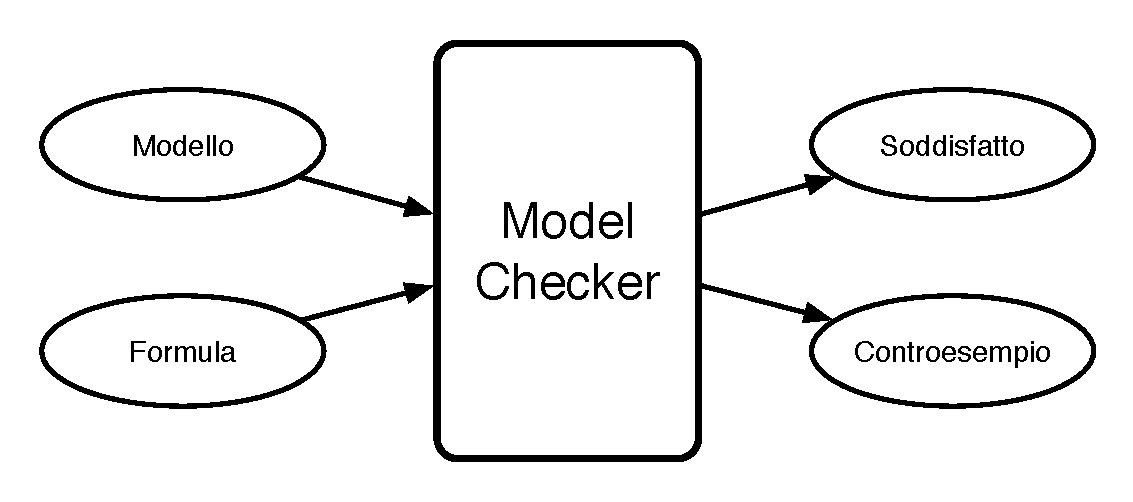
\includegraphics[width=.8\textwidth]{Images/mc.eps}
	\end{center}
\caption{Schema del funzionamento di un model checker}
\label{fig:modelchecker}
\end{figure}

In un contesto reale è spesso impossibile pensare di ottenere un sistema complesso totalmente privo di errori o imperfezioni, si rilassano quindi le richieste introducendo dei gradi di tolleranza degli errori. Un caso concreto può essere il gestore di una compagnia telefonica che permette di effettuare un'alta percentuale di chiamate senza problemi di interferenze o interruzioni, ad esempio il $98\%$. Oltre al modello e alla formula viene quindi introdotto nel model checker il parametro dell'\emph{accuratezza} che rende una formula verificata se il grado di fallimento rientra nella tolleranza espressa. Un model checker a cui si aggiunge un parametro di accuratezza espresso in probabilità viene chiamato \emph{probabilistic model checker} (figura \ref{fig:probabilisticmodelchecker}).
\begin{figure}[htb]
	\begin{center}
		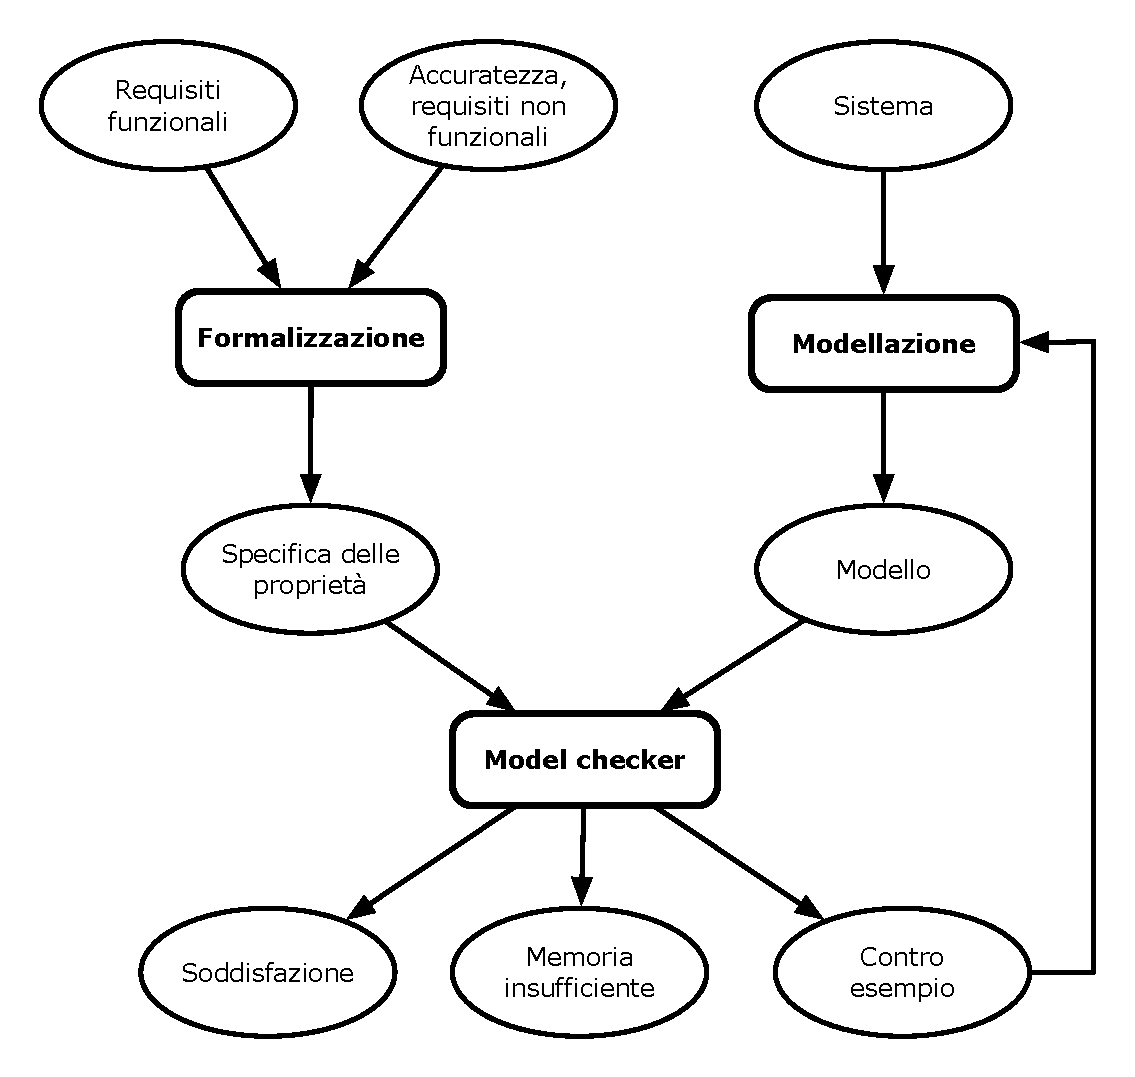
\includegraphics[width=\textwidth]{Images/pmc.eps}
	\end{center}
\caption{Schema del funzionamento di un model checker probabilistico}
\label{fig:probabilisticmodelchecker}
\end{figure}

Dalla formalizzazione dei requisiti si può ottenere un insieme di proprietà che dovranno essere soddisfatte. Più precisamente, dai requisiti \emph{funzionali} possiamo ottenere le formule di proprietà da soddisfare, mentre quelli \emph{non funzionali} forniscono l'accuratezza da utilizzare. Dopo aver fornito al model checker il modello del sistema, la proprietà da verificare e l'accuratezza, questo può produrre tre tipi di risposte:
\begin{itemize}
	\item la proprietà viene soddisfatta dal modello nei limiti richiesti,
	\item la memoria non è sufficiente per portare a termine la verifica oppure
	\item la proprietà non viene soddisfatta dal modello, fornendo un controesempio.
\end{itemize}
Se non si riceve esito positivo si può intervenire a seconda di che tipo di problema è stato riscontrato. Nel secondo caso si verifica il fenomeno conosciuto come \emph{esplosione degli stati} che ha origine quando si vuole modellare sistemi molto complessi, come i già citati software multithread. La conseguenza è una richiesta di memoria e tempo di calcolo proibitivi. Per far fronte a questo problema si ricorre spesso alla scomposizione del sistema in sotto sistemi e ad astrazioni di modelli troppo complessi. Ovviamente se invece non viene soddisfatta la formula è necessario intervenire sul modello stesso cercando di correggere i comportamenti erronei evidenziati.

Il model checking viene utilizzato in modo diverso se ci troviamo prima o dopo la fase di sviluppo: nel primo caso è necessario costruire il modello astratto del sistema, nel secondo, invece, è possibile utilizzare degli strumenti (i.e. \emph{java path finder}) per effettuare le verifiche direttamente sul codice. 

\section{Probabilit\`a elementari}
Introduciamo le misure principali utilizzate dei model checker probabilistici, assumendo di utilizzare come strutture dei modelli le \ac{dtmc} e le \ac{mdp}. Esistono due tipi di misure di probabilità elementari delle \ac{dtmc}:
\begin{itemize}
	\item probabilità \emph{transiente} e
	\item probabilità \emph{a regime}, o \emph{steady state}.
\end{itemize}

\begin{mtdef}[Probabilità transiente $\pi_j(n)$]
La probabilità \emph{transiente} $\pi_j(n) = \mathbb{P}\{X_n = j\}$ è la probabilità che la \ac{dtmc} sia nello stato $j$ al passo $n$
\end{mtdef}

Possiamo quindi associare alla \ac{dtmc} $\mathcal{D}$ un vettore che al passo $n$ descriva la probabilità di trovarsi in ogni stato $s \in S$ $$\underline\pi(n) \triangleq (\pi_1(n), \dots, \pi_{|S|}(n)).$$
Si indica con $\underline\pi(0)$ la distribuzione di probabilità iniziale mentre con $\underline\pi(n)$ la distribuzione di probabilità al passo $n$.
Considerando che moltiplicare il vettore di distribuzione di probabilità per la matrice $\mathbb{P}$ rappresenta un avanzamento del sistema che aggiorna la distribuzione al passo successivo, allora vale la seguente \emph{relazione di ricorrenza}
$$ \underline\pi(n) = \underline\pi(n-1) \cdot \mathbb{P} $$
da cui si ricava immediatamente la seguente forma dipendente solo dalla  distribuzione iniziale e dalla matrice di transizione
$$ \underline\pi(n) = \underline\pi(0) \cdot \mathbb{P}^n$$

\begin{mtdef}[Probabilità steady state $\pi_j$]
La probabilità \emph{steady state} $$\pi_j = \lim_{n\rightarrow\infty} \mathbb{P}\{X_n = j\}$$ è la probabilità che la \ac{dtmc} sia a regime nello stato $j$.
\end{mtdef}

L'esistenza di questo limite è garantita solo sotto determinate condizioni di \emph{ergodicità} della catena. Supponendo che il limite sia indipendente dalla distribuzione iniziale, per calcolare questa distribuzione è sufficiente risolvere il seguente sistema di equazioni lineari
$$
\left\{
\begin{array}{l}
\underline\pi \cdot \mathbb{P} = \underline\pi \\
\sum^{|S|}_{i=1} \pi_i = 1 \\
\end{array}
\right.
$$
dove $0 \leq \pi_i \leq 1$ e $1 \leq i \leq |S|$.

Una volta scelto uno scheduler che risolva le scelte nondeterministiche della \ac{mdp} trasformandola in una \ac{dtmc} sarà possibile applicare la valutazione delle probabilità sopra descritte. Il risultato però sarà valido solo in presenza di quello specifico scheduler che potrebbe avere un peso poco rilevante nell'analisi della \ac{mdp}. Quello che si fa quindi è calcolare il range di probabilità in cui si muove la misura interessata \emph{per ogni} possibile scheduler in modo da poter fare inferenza su \emph{lower} e \emph{upper bounds}.

\section{Probabilistic Computation Tree Logic}
Al fine di poter effettuare model checking su strutture come \ac{dtmc} e \ac{mdp} utilizziamo \ac{pctl}, un'estensione probabilistica della logica temporale \ac{ctl}. Il linguaggio \ac{pctl} è uno strumento che permette di esprimere specifiche di interesse sulla struttura che stiamo condiderando. Può essere quindi utilizzato sia sulle \ac{dtmc} che sulle \ac{mdp} adattando la struttura alla potenza espressiva del modello. In generale le formule che esprimono specifiche in modo formale hanno un ruolo fondamentale all'interno del model checking in quanto permettono di rendere automatico il procedimento di verifica.

In seguito riportiamo la sintassi e la semantica di \ac{pctl} definita per le \ac{mdp}, più generale rispetto a quella per le \ac{dtmc} ed effettivamente impiegata all'interno di questo lavoro.

\begin{mtdef}[Sintassi \ac{pctl}]
	La sintassi \ac{pctl} viene definita come segue:
$$
\begin{array}{rcl}
	\phi &::=& true \Sep \mathit{a} \Sep \phi_1 \wedge \phi_2 \Sep \neg\phi \Sep \mathcal{P}_{\bowtie p}[\psi] \\
	\psi &::=& \mathcal{X}\phi \Sep \phi_1 \mathcal{U}^{\leq k} \phi_2 \Sep \phi_1 \mathcal{U} \phi_2 \\
\end{array}
$$
dove $\mathit{a}$ è una proposizione atomica, $\bowtie \in \{\leq,<,\geq,>\}$, $p \in[0,1]$ e $k \in \mathbb{N}$.
\end{mtdef}
Dalla sintassi distinguiamo due tipi di formula: le formule di stato $\phi$ e le formule di cammino $\psi$. Per definire formalmente la semantica è necessario specificare come gli elementi dell'insieme $AP$ delle proposizioni atomiche sono gestiti in una \ac{mdp}.
\begin{mtdef}[\ac{mdp} etichettata]
	Una \ac{mdp} etichettata è una tupla $(\mathcal{M},L)$ dove:
	\begin{itemize}
		\item $\mathcal{M}$ è una \ac{mdp};
		\item $L:S\rightarrow 2^{AP}$ è una funzione di etichettatura.
	\end{itemize}
\end{mtdef}
Estendiamo quindi la struttura delle \ac{mdp} con una funzione $L$ che associa ad ogni stato un certo insieme di proposizioni atomiche. A questo punto abbiamo tutti gli strumenti per definire la semantica di \ac{pctl} secondo una relazione di soddisfacibilità.
\begin{mtdef}[Relazione di soddisfacibilità]
	Sia $\mathcal{M} = (S,\overline{s},Act,Steps,L)$ una \ac{mdp} etichettata. Per ogni stato $s \in S$, la relazione di soddisfacibilità di stato $\models$ è definita per induzione come segue:
$$
	\begin{array}{rllcl}
		\mathcal{M},s &\models& \phi &\Leftrightarrow& \mathcal{M},s \models_{st} \phi \\
		\mathcal{M},s &\models_{st}& true && \forall s \in S, \\
		\mathcal{M},s &\models_{st}& \mathit{a} &\Leftrightarrow& \mathit{a} \in L(s), \\
		\mathcal{M},s &\models_{st}& \neg\phi &\Leftrightarrow& s \not\models_{st} \phi, \\
		\mathcal{M},s &\models_{st}& \phi_1 \wedge \phi_2 &\Leftrightarrow& s\models_{st}\phi_1 \ e\ s\models_{st}\phi_2, \\
		\mathcal{M},s &\models_{st}& \mathbb{P}\{ \mathcal{P}_{\bowtie p}[\psi]\} &\Leftrightarrow& p_s^\Sigma(\psi)\bowtie p,\ \forall\ \Sigma \in Scheduler_\mathcal{M}, \\
	\end{array}
$$
dove per ogni scheduler $\Sigma \in Scheduler_\mathcal{M}$:
$$
p_s^\Sigma \triangleq Prob_s^\Sigma(\{\pi \in Path_s^\Sigma \sep \pi \models_{pt} \psi\})
$$
e per ogni cammino $\pi \in Path$:
$$
\begin{array}{rclcl}
	\mathcal{M},\pi & \models_{pt} & \mathcal{X}\phi & \Leftrightarrow & \mathcal{M},\pi(1) \models_{pt} \phi, \\
	\mathcal{M},\pi & \models_{pt} & \phi_1 \mathcal{U}^{\leq k} \phi_2 & \Leftrightarrow & \exists i \leq k\ .\ (\mathcal{M},\pi(i) \models_{pt} \phi_2\ e\ \mathcal{M},\pi(j) \models_{pt} \phi_1 \forall j < i), \\
	\mathcal{M},\pi & \models_{pt} & \phi_1 \mathcal{U} \phi_2 & \Leftrightarrow & \exists k \geq 0\ .\ \mathcal{M},\pi \models_{pt} \phi_1 \mathcal{U}^{\leq k} \phi_2. \\
\end{array}
$$
\end{mtdef}

Per specificare una formula \ac{pctl} si utilizza sempre una formula di stato che al suo interno potrà utilizzare formule di cammino. Intuitivamente gli operatori logici possono essere utilizzati per indagare sulle proposizioni atomiche contenute in un determinato stato, mentre l'operatore $\mathcal{P}_{\bowtie p}[\psi]$ viene soddisfatto dagli stati che soddisfano la formula di cammino $\psi$ con una probabilità nell'intervallo specificato da $\bowtie p$. Questo operatore si comporta sempre nel modo appena descritto se i cammini non incontrano scelte nondeterministiche (nelle \ac{dtmc} è sempre vero) ma come deve comportarsi in caso contrario? Dato che non si può assumere niente sulle suddette scelte e sfruttando il fatto che l'applicazione di uno scheduler ad una \ac{mdp} produce una \ac{dtmc}, l'operatore è considerato soddisfatto se la condizione è valida \emph{per qualsiasi scheduler}.

Per quanto riguarda le formule di cammino, l'operatore \emph{next} $\mathcal{X}\phi$ richiede che $\phi$ venga soddisfatta dallo stato successivo, l'operatore \emph{bounded until} $\phi_1 \mathcal{U}^{\leq k} \phi_2$ richiede che $\phi_2$ venga soddisfatto entro $k$ passi e che $\phi_1$ resti sempre soddisfatto fino a quel punto, mentre l'operatore \emph{unbonded until} $\phi_1 \mathcal{U} \phi_2$ richiede che prima o poi $\phi_2$ venga soddisfatto e che $\phi_1$ sia sempre soddisfatto fino a quel punto.

Possiamo rielaborare i construtti principali definiti finora per estendere il linguaggio con degli operatori derivati (tabella \ref{tab:sintassi:derivati}). Mentre gli operatori logici $false$, $\vee$ e $\rightarrow$ possono essere derivati facilmente, vi sono alcuni operatori meno banali. Gli operatori $\Diamond$ e $\Box$ sono molto comuni nelle logiche temporali e servono a specificare rispettivamente proprietà che hanno speranza di avverarsi in futuro e proprietà che sicuramente non si verificheranno mai. Delle applicazioni interessanti di questi due concetti sono le proprietà di \emph{liveness} e di \emph{safety}. Una proprietà di \emph{liveness} esprime la possibilità che prima o poi accada qualcosa di positivo mentre la duale \emph{safety} indica che qualcosa di negativo non potrà mai accadere. I due operatori possono essere usati per descrivere queste due tipologie proprietà ma sono più generali. 
Le varianti \emph{bounded} $\Diamond^{\leq k}$ e $\Box^{\leq k}$ stabiliscono, tramite il numero di passi $k \in \mathbb{N}$, il tempo entro il quale la proprietà $\phi$ deve rimanere soddisfatta a partire dall'istante iniziale. La proprietà di cammino $\Diamond^{\leq k}\phi$ sarà quindi soddisfatta se entro $k$ passi $\phi$ si verificherà almeno una volta, mentre la proprietà di cammino $\Box^{\leq k}$ sarà soddisfatta se $\phi$ rimarrà sempre soddisfatta per tutti e $k$ i passi. 
Per definire gli operatori $\Box$ e $\Box^{\leq k}$ viene introdotta la notazione $\overline\bowtie$ che rappresenta l'inversione degli operatori secondo le seguenti equivalenze: $\overline\leq \equiv \geq$, $\overline < \equiv >$, $\overline\geq \equiv \leq$ e $\overline > \equiv <$.
Un ultimo operatore interessante è il quantificatore esistenziale $\exists$ che \emph{ricerca l'esistenza di uno scheduler} che soddisfa una certa formula, contrariamente all'approccio generale basato sulla soddisfacibilità di tutti i possibili scheduler.
\begin{table}[htbp!]
$$
\begin{array}{rcl}
	false & \equiv & \neg true \\
	\phi_1 \vee \phi_2 & \equiv & \neg(\neg\phi_1 \wedge \neg\phi_2) \\
	\phi_1 \rightarrow \phi_2 & \equiv & \neg\phi_1 \vee \phi_2 \\
	\mathcal{P}_{\bowtie p}[\Diamond \phi] & \equiv & \mathcal{P}_{\bowtie p}[true \mathcal{U} \phi] \\
	\mathcal{P}_{\bowtie p}[\Diamond^{\leq k} \phi] & \equiv & \mathcal{P}_{\bowtie p}[true \mathcal{U}^{\leq k} \phi] \\
	\mathcal{P}_{\bowtie p}[\Box \phi] & \equiv & \mathcal{P}_{\overline\bowtie 1-p}[\Diamond \neg \phi] \\
	\mathcal{P}_{\bowtie p}[\Box^{\leq k} \phi] & \equiv & \mathcal{P}_{\overline\bowtie 1-p}[\Diamond^{\leq k} \neg \phi] \\
	\exists\Diamond\phi & \equiv & \neg \mathcal{P}_{\leq 0}[\Diamond\phi] \\
\end{array}
$$
\caption{Operatori derivati di \acs{pctl}}
\label{tab:sintassi:derivati}
\end{table}

\section{PRISM model checker}
Il model checker probabilistico che utilizzeremo è \prism{} \cite{KNP11}. Si tratta di un tool con il quale è possibile fare modellazione e analisi di sistemi che presentano aspetti probabilistici. I principali modelli probabilistici supportati sono le \ac{dtmc}, le \ac{mdp}, le \ac{ctmc} ed i \ac{pta}, mentre i linguaggi utilizzabili per descrivere le formule sono \ac{pctl}, \ac{csl} e \ac{ltl}. In questa sezione descriveremo l'utilizzo di \prism{} concentrandoci sugli strumenti di interesse diretto per questo lavoro come le \ac{mdp} e il linguaggio \ac{pctl} precedentemente descritti.

\prism{} utilizza un suo specifico linguaggio con il quale è possibile definire tutti i modelli sopra citati. Si tratta infatti di un linguaggio basato sugli stati e su formalismi tipici dei sistemi reattivi. I componenti fondamentali rappresentati dal linguaggio sono i \emph{moduli} e le \emph{variabili}, un \emph{modello} viene rappresentato come un insieme di moduli che possono interagire tra loro. Ogni modulo può inoltre contenere delle variabili locali e il valore di queste variabili ad un certo istante rappresentano il suo stato. Allo stesso modo lo stato del modello globale è definito come lo stato locale di tutti i moduli che lo compongono.

Il comportamento di un modulo viene definito dall'insieme di \emph{comandi} che contiene. Un comando ha la seguente forma:
\begin{verbatim}
	[] guardia -> prob_1 : update_1 + ... + prob_n : update_n ;
\end{verbatim}
La \emph{guardia} è un predicato che può considerare qualsiasi variabile del modello e se risulta soddisfatta il modello può avanzare eseguendo una delle transizioni \emph{update} con le rispettive probabilità (o evenutalmente rate). L'intero modulo viene definito specificandone il nome e il contenuto
\begin{verbatim}
	module name ... endmodule
\end{verbatim}
All'interno del modulo possono essere presenti sia comandi che variabili. Al fine di avere uno \emph{spazio finito di stati} \prism{} permette di gestire solo variabili booleane e variabili intere in un range finito. Di seguito mostriamo la dichiarazione di una variabile $x$ che può assumere i valori interi compresi tra $0$ e $10$ compresi inizializzata a 5 e una variabile booleana $b$ inizializzata a $true$:
\begin{verbatim}
	x : [0..10] init 5;
	b : bool init true;
\end{verbatim}
Le guardie sono classiche espressioni booleane che possono fare riferimento a variabili di qualsiasi modulo in quanto viene richiesta solamente la lettura dei valori. Gli update, invece, sono sequenze di assegnamenti intervallate dal separatore $\&$. La sequenza di update vuota viene indicata con $true$. Un assegnamento di un valore a una variabile può avvenire solo su una variabile locale al modulo a cui appartiene il comando, inoltre il nome della variabile aggiornata deve terminare col simbolo $'$ ad indicarne il nuovo stato. All'interno del listato \ref{code:prism:example1} mostriamo l'utilizzo degli strumenti appena descritti. L'esempio rappresenta due processi in mutua esclusione.
\begin{lstlisting}[language=prism,style=eclipse,caption={Esempio di definizione dei moduli in \prism{}},label=code:prism:example1]
module M1

x : [0..2] init 0;

    [] x=0 -> 0.8:(x'=0) + 0.2:(x'=1);
    [] x=1 & y!=2 -> (x'=2);
    [] x=2 -> 0.5:(x'=2) + 0.5:(x'=0);

endmodule 

module M2

y : [0..2] init 0;

    [] y=0 -> 0.8:(y'=0) + 0.2:(y'=1);
    [] y=1 & x!=2 -> (y'=2);
    [] y=2 -> 0.5:(y'=2) + 0.5:(y'=0);

endmodule
\end{lstlisting}
In questo caso i due moduli sono simmetrici, ed entrambi presentano esclusivamente scelte probabilistiche. Possiamo se necessario inserire anche delle scelte non deterministiche sulle quali è quindi impossibile fare osservazioni di tipo quantitativo. Modificando il modulo $M1$ come mostrato nel listato \ref{code:prism:example2} inseriamo una scelta nondeterministica, infatti le due nuove guardie insierite saranno sempre abilitate insieme.
\begin{lstlisting}[language=prism,style=eclipse,caption={Scelta nondeterministica in \prism{}},label=code:prism:example2]
module M1

x : [0..2] init 0;

	// scelta nondeterministica
    [] x=0 -> (x'=0);
	[] x=0 -> (x'=1);
	
    [] x=1 & y!=2 -> (x'=2);
    [] x=2 -> 0.5:(x'=2) + 0.5:(x'=0);
	
endmodule
\end{lstlisting}
In generale il nondeterminismo può verificarsi anche se due guardie vengono soddisfatte assieme anche solo parzialmente. La stessa struttura può quindi presentare scelte deterministiche a seconda dello stato corrente.

In \prism{} è anche possibile definire delle costanti globali sui domini di interi, reali e booleani:
\begin{verbatim}
	const int z = 12;
	const double pi = 3.141592;
	const bool flag = true;
\end{verbatim}
Queste costanti possono essere utilizzate, al fine di parametrizzare il modello, all'interno delle espressioni che possono coinvolgere i seguenti operatori:
\begin{itemize}
	\item $-$ meno unario, $*$ moltiplicazione, $\slash$ divisione, $+$ somma e $-$ sottrazione,
	\item le relazioni d'ordine $<$, $\leq$, $>$, $\geq$, e di equivalenza $=$ e $!=$
	\item gli operatori booleani di $!$ negazione, $\&$ congiunzione, $|$ disgiunzione, $<=>$ se e solo se e $=>$ implicazione logica.
\end{itemize}
Sono presenti inoltre le funzioni:
\begin{itemize}
	\item $min$ minimo e $max$ massimo,
	\item $floor$ di arrotondamento all'intero minore più vicino,
	\item $ceil$ di arrotondamento all'intero maggiore più vicino,
	\item $pow$ per l'elevamento a potenza,
	\item $mod$ modulo,
	\item $log$ logaritmo.
\end{itemize}
Le espressioni possono essere utilizzate non solo nelle condizioni delle guardie, nelle inizializzazioni e negli aggiornamenti, ma anche per calcolare le proprietà di una transizione.

Come primo parametro di un comando può essere inserita la label di un'azione per far sincronizzare i moduli. Un azione viene quindi specificata inserendone il nome (ad esempio \emph{step}) all'interno delle parentesi quadre, nel seguente modo
\begin{verbatim}
	[step] x=0 -> 0.8:(x'=0) + 0.2:(x'=1);
\end{verbatim}

Il modello finale viene ricavato di default dalla \emph{composizione parallela} di tutti i moduli che lo compongono, se si vuole invece descrivere una composizione diversa, è possibile usare il costrutto
\begin{verbatim}
	system ... endsystem
\end{verbatim}
Al suo interno possono essere usati i seguenti operatori \ac{csp}:
\begin{itemize}
	\item $M1\ ||\ M2$: i moduli si sincronizzano solo su azioni che appaiono in entrambi (composizione parallela di default),
	\item $M1\ |||\ M2$: interleaving completo, senza sincronizzazione,
	\item $M1\ |[a,b,...]|\ M2$: la sincronizzazione avviene solo sulle azioni specificate nell'operatore,
	\item $M \slash \{a,b,...\}$ le azioni specificate vengono nascoste all'esterno,
	\item $M \{a<-b,c<-d,...\}$ le azioni vengono rinominate all'esterno.
\end{itemize}
Alcuni esempi di espressioni di sistema sono mostrati di seguito:
\begin{verbatim}
	system (station1 ||| station2 ||| station3) |[serve]| server endsystem
	system ((P1 |[a]| P2) / {a}) || Q endsystem
	system ((P1 |[a]| P2) {a<-b}) |[b]| Q endsystem
\end{verbatim}

%!TEX root = ../main.tex

\myChapter{PRISM}
\cleardoublepage\myPart{LAPSA: un linguaggio per agenti adattivi}
\documentclass{article}

\title{SEAL: Self Adaptive Agents Specific Language}
\author{Marco Tinacci}
\date{\today}

\usepackage[italian]{babel} % lingua italiana
\usepackage[utf8]{inputenc} % codifica per caratteri con accento
\usepackage{latexsym} % join symbol
\usepackage{amsmath} % x right arrow
\usepackage{amssymb} % triangle equivalence symbol
% MACRO
\newcommand{\Sep}{\quad\mid\quad}
\newcommand{\Space}{\mbox{ }}
\newcommand{\Par}{\Space||_A\Space}

\begin{document}
\maketitle
\tableofcontents
\section{Syntax}

$$
\begin{array}{|rcl@{\ \ }l|}
\hline
S &::=& m \Sep S \Par S & \mbox{(System)} \\
\gamma &::=& \beta \Rightarrow \delta \Sep \gamma,\gamma & \mbox{(Rule)} \\
\beta &::=& \exists \Space m \Space x: (\beta) \Sep e \Join e \Sep \mathbf{tt} \Sep \beta \vee \beta \Sep \neg\beta & \mbox{(Condition)} \\
\delta &::=& <e,a> \alpha \Sep \delta \oplus \delta & \mbox{(Distribution)} \\
\alpha &::=& x = e; \Sep \mathbf{no action}; \Sep \alpha \Space \alpha & \mbox{(Action)} \\
\hline
\end{array}
$$

Sono state omesse le descrizioni di alcuni simboli per alleggerire la lettura della sintassi:
\begin{itemize}
	\item $m$: riferimento alla definizione di un modulo,
	\item $A$: insieme di azioni di sincronizzazione,
	\item $e$: espressione,
	\item $\Join$: operatore di confronto,
	\item $x$: dichiarazione di un identificatore,
	\item $a$: label azione.
\end{itemize}

\subsection{Syntactic sugar}
Inseriamo un costrutto tale da poter inserire una condizione di abilitazione sugli elementi del supporto della distribuzione:
$$
\beta \Rightarrow <e,a,\beta'> \alpha \oplus \delta
\equiv 
\beta \wedge \beta' \Rightarrow <e,a> \alpha \oplus \delta,
\beta \wedge \neg\beta' \Rightarrow \delta
$$


\section{Semantic}
Andiamo a dare un'introduzione informale alla semantica del linguaggio descritto:
\begin{itemize}
	\item \emph{System}: un sistema può essere definito tramite un singolo modulo ($m$ è un riferimento alla definizione di un modulo) o attraverso la composizione parallela di più sistemi su di un insieme di azioni di sincronizzazione $A \subseteq Act$;
	\item \emph{Rule}: un insieme di regole definisce il comportamento di un modulo, se vale la condizione $\beta$ si può passare alla valutazione della distribuzione $\delta$;
	\item \emph{Condition}: descrive una condizione fornendo anche un operatore di quantificatore esistenziale sui moduli;
	\item \emph{Distribution}: descrive una distribuzione probabilistica di azioni $\alpha$, dove ogni azione è accompagnata da un'espressione $e$, che ne descrive il peso, e un'azione $a$;
	\item \emph{Action}: un azione descrive un aggiornamento dello stato, che può consistere nell'assegnamento di una, nessuna, o più variabili.
\end{itemize}

Definiamo la semantica del linguaggio in termini di \emph{Markov Decision Processes}. Alla definizione di ogni modulo sarà assegnata una \emph{MDP} della forma:
$$ (\Sigma,Act,\rightarrow_\rho,\sigma_0) $$
dove 
\begin{itemize}
	\item $\Sigma \triangleq \{\sigma | \sigma : \mathbb{VAR} \rightarrow \mathbb{VAL}\}$ è l'insieme degli \emph{stati} rappresentati da funzioni che mappano variabili in valori,
	\item $Act$ l'insieme delle azioni,
	\item $\rightarrow_\rho \subseteq \Sigma \times Act \times Dist(U)$ è la relazione di \emph{avanzamento} di stato,
	\item $\sigma_0 \in \Sigma$ è lo \emph{stato iniziale},
	\item $\rho \subseteq \beta \times Act \times 2^{Dist(U)}$ è la \emph{struttura statica} del \emph{MDP},
	\item $U \triangleq \{u | u : \Sigma \rightarrow \Sigma \}$ è l'insieme delle funzioni \emph{update} di aggiornamento di stato.
\end{itemize}



$$
\begin{array}{cl}
	\displaystyle{\frac{(g,a,\mathcal{D}) \in \rho}{\sigma \xrightarrow{a}_\rho d(\sigma)} \Space \sigma \models g, d \in \mathcal{D} } & \mbox{(Update)} \\
\end{array}
$$

$$
\begin{array}{|cl|}
	\hline
	\displaystyle{\frac{S_1 \xrightarrow{a} \Pi_1 \quad S_2 \xrightarrow{a}_\rho \Pi_2}{S_1 \Par S_2 \xrightarrow{a} \Pi_1 \Par \Pi_2}a \in A} & \mbox{(Sync)} \\[.5cm]
	\displaystyle{\frac{S_1 \xrightarrow{a} \Pi_1}{S_1 \Par S_2 \xrightarrow{a}_\rho \Pi_1 \Par S_2}a \not\in A} & \mbox{(Async\ 1)} \\[.5cm]
	\displaystyle{\frac{S_2 \xrightarrow{a} \Pi_2}{S_1 \Par S_2 \xrightarrow{a}_\rho S_1 \Par \Pi_2}a \not\in A} & \mbox{(Async\ 2)} \\[.5cm]
	\hline
\end{array}
$$


\section{Examples}
Esempio di un modulo di robot che esegue una \emph{random walk} su una griglia escludedo dalla scelta probabilistica le direzioni adiacenti occupate:
$$
\begin{array}{rcl}
m_1 & \triangleq & \mathbf{tt} \Rightarrow \\ 
	& & <1, north, \neg \Space \exists \Space m_1 \Space v: v.x=x \wedge v.y=y+1> y=y+1; \oplus \\
	& & <1, south, \neg \Space \exists \Space m_1 \Space v: v.x=x \wedge v.y=y-1> y=y-1; \oplus \\ 
	& & <1, east, \neg \Space \exists \Space m_1 \Space v: v.x=x+1 \wedge v.y=y> x=x+1; \oplus \\ 
	& & <1, west, \neg \Space \exists \Space m_1 \Space v: v.x=x-1 \wedge v.y=y> x=x-1; \oplus \\ 
	& & <1, stay, \mathbf{tt}> \mathbf{noaction};\\ 
\end{array}
$$
Esempio di un modulo di robot analogo al precedente con la differenza che la scelta della mossa viene fatta in modo nondeterministico:
$$
\begin{array}{rclcl}
m_2 & \triangleq & \neg \Space \exists \Space m_1 \Space v: (v.x=x \wedge v.y=y+1) &\Rightarrow& <1,north> y=y+1; \\ 
	& & \neg \Space \exists \Space m_1 \Space v: (v.x=x \wedge v.y=y-1) &\Rightarrow& <1,south> y=y-1; \\ 
	& & \neg \Space \exists \Space m_1 \Space v: (v.x=x+1 \wedge v.y=y) &\Rightarrow& <1,east> x=x+1; \\ 
	& & \neg \Space \exists \Space m_1 \Space v: (v.x=x-1 \wedge v.y=y) &\Rightarrow& <1,west> x=x-1; \\ 
	& & \mathbf{tt} &\Rightarrow& <1,stay> \mathbf{noaction}; \\ 
\end{array}
$$

\end{document}

\cleardoublepage\myPart{Caso di studio}
%!TEX root = ../main.tex

\chapter{Caso di studio}

% TODO riferimento ai lavori di Del Toro sui robot che si muovono sulla griglia

% descrizione dello scenario
Lo scenario preso come caso di studio prevede una popolazione di agenti mobili che si muovono casualmente all'interno di un'area limitata. Gli agenti possono venire a conoscenza, tramite dei sensori di prossimità, della presenza di altri agenti entro un raggio limitato.
Ogni singolo agente può decidere periodicamente se muoversi verso nord, sud, est o ovest o se stare fermo.
L’obiettivo primario è quello di associare uno scheduler all'agente protagonista che minimizzi il numero di collisioni con altri agenti che si verificheranno.

\section{Analisi}
Per l’analisi del problema vengono effettuate le seguenti assunzioni:
\begin{itemize}
	\item ogni agente si può muovere solo nelle quattro direzioni (nord, sud, ovest, est) o può decidere di rimanere fermo,
	\item tutti gli agenti sono \emph{sincronizzati nello spazio}: esiste una griglia globlale che rappresenta le strade percorribili dagli agenti,
	\item tutti gli agenti sono \emph{sincronizzati nel tempo}: tutti eseguono allo stesso tempo un passo nella direzione scelta.
\end{itemize}

Possiamo quindi rappresentare la zona con una matrice $Z \in \mathbb{N}_0^{m\cdot m}$, dove $m \in \mathbb{N}$ indica la dimensione della zona e gli elementi della matrice indicano il numero di agenti in una certa posizione. Se $Z_{i,j}=0$ la posizione è \emph{libera}, se $Z_{i,j}=1$  allora la posizione è \emph{occupata} da un agente, mentre se $Z_{i,j}>1$ allora in quella posizione si sta verificando una \emph{collisione}.

Per analizzare la successione temporale dello scenario possiamo parametrizzare la matrice $Z$ rispetto al tempo definendola come una funzione $Z:\mathbb{N}_0 \rightarrow \mathbb{N}^{m\cdot m}$ che, dato un certo istante temporale $n \in \mathbb{N}_0$, restituisce una matrice $Z(n)$ che descrive la zona in quell’istante. Lo scenario iniziale è rappresentato da $Z(0)$.
Assumendo che i sensori di un agente permettano di rilevare se un altro agente si trova entro un passo di distanza, definiamo le \emph{posizioni adiacenti} come le posizioni raggiungibili all’interno della zona che non portino ad uno scontro diretto con un altro agente:
$$ N_{i,j} = \{(i',j') : |i-i'+j-j'| = 1 \wedge i',j' \in \{1,\dots,m\}\} \cup \{(i,j)\} $$.

Il criterio seguito dal generico agente sarà quindi l'algoritmo \ref{alg:scelta}.
\begin{algorithm}
	\caption{Algoritmo di scelta generico}
	\label{alg:scelta}
	\begin{algorithmic}
		\REQUIRE $m,n,nrob \in \mathbb{N} \wedge i,j \in \{1,\dots,m\} \wedge Z \in \mathbb{N}_0^{m\cdot m} $
		\STATE $p_0 = (i,j)$
		\FOR{$k=1$ \TO $n$}
			\STATE $p_k = schedule(local(Z,p_{k-1},m),m,nrob)$
			\STATE \emph{barriera}
			\STATE $Z_{p_{k-1}} = Z_{p_{k-1}} - 1$
			\STATE $Z_{p_{k}} = Z_{p_{k}} + 1$
			\STATE \emph{barriera}
		\ENDFOR
	\end{algorithmic}
\end{algorithm}
I parametri dell'algoritmo hanno il seguente significato:
\begin{itemize}
	\item $m$ è la dimensione dell'area,
	\item $n$ è il numero di passi che vengono eseguiti da ogni agente (generalmente possiamo immaginarlo come un numero molto grande),
	\item $nrob$ è il numero di agenti presenti nell'area,
	\item $i$ e $j$ sono la posizione iniziale dell'agente,
	\item $Z$ è lo stato iniziale della matrice globale.
\end{itemize}

La funzione \emph{local} viene così definita
$$ local(Z,i,j,m) = Z[I(i,m),J(j,m)] $$
Il primo sottoinsieme di indici è definito come
$$ I(i,m) =
\left\{
\begin{array}{ll}
	\{i, i+1\} & \mbox{se } i = 1 \\
	\{i-1, i\} & \mbox{se } i = m \\
	\{i-1, i, i+1\} & \mbox{altrimenti} \\
\end{array}
\right.
$$
e il secondo, in modo analogo $J(j,m) = I(j,m)$. Con la funzione \emph{local} si vuole definire formalmente la sottomatrice locale che viene rilevata dal sensore di prossimità dell'agente.

La funzione \emph{schedule} dipende invece dal comportamento che si vuole associare all'agente e quindi che criterio utilizzerà per risolvere le scelte. Lo scheduler avrà quindi pochi dati su cui prendere una decisione e se si esclude anche una memorizzazione dello storico allora il dominio di \emph{schedule} diventa il numero di combinazioni di un massimo di $nrob$ agenti all'interno delle posizioni locali. La conoscenza dell'agente si limita quindi alle posizioni locali $local(Z,i,j,m)$, il numero totale di agenti in gioco $nrob$ e la dimensione dell'area $m$.

Le \emph{barriere} sono il costrutto di programmazione parallela dove ogni agente attende che tutti gli altri abbiano raggiunto il suo stesso punto, dopodichè tutti possono riprendere l'esecusione. In questo caso vengono utilizzate per un doppio scopo: il primo è di evitare la \emph{race condition} e il secondo e quello di avere una separazione netta tra le fasi globali di decisione del prossimo passo e aggiornamento della mappa.

\section{Approcci proposti}
Introduciamo i due principali algoritmi di scheduling utilizzati in questo caso di studio:
\begin{itemize}
	\item semi-casuale,
	\item basato sul model-checking.
\end{itemize}
Lo scheduling \emph{semi-causale} non fa altro che scegliere casualmente una delle posizioni libere raggiungibili al prossimo passo.

Lo scheduling basato sul model-checking, invece, è incentrato sulla costruzione di un modello globale ottenuto facendo ipotesi sugli aspetti che non si conoscono. Una volta che si ha a disposizione il modello globale ``stimato'' si procede valutando la probabilità di soddisfare la formula che rappresenta l'obiettivo nel caso in cui si effettua una determinata scelta tramite model-checking.

In questo caso di studio si conosce quanti agenti sono presenti ma non il loro comportamento e con che criterio prediligono una direzione piuttosto che un'altra. Si ipotizza il movimento degli altri agenti come uno scheduling casuale che, a differenza di quello semi-casuale, può scegliere anche direzioni occupate da altri agenti vietando comunque direzioni che farebbero uscire dal perimetro dell'arena. Il modello globale viene quindi correttamente rappresentato da una \ac{mdp} in quanto è composizione parallela dei modelli degli agenti contenenti scelte nondeterministiche e probabilistiche.

Assumiamo l'implementazione in \ac{lapsa} dello scheduler dell'agente mostrata nel listato \ref{code:lapsa_agent}, ipotizzando che esista solo un altro agente nell'area e che questo si muova secondo uno scheduler casuale:
\begin{itemize}
	\item ogni variabile indica se una posizione è occupata da un altro agente (valore $1$) o libera (valore $0$), la posizione \texttt{p1} indica l'area a nord-ovest, \texttt{p2} quella a nord, fino alla \texttt{p9} che è quella a sud-est,
	\item la posizione \texttt{p5} è l'area interna di collisione con l'agente, se altri agenti vengono rivelati in quella zona lo stato viene interpretato come collisione, per questo motivo l'obiettivo dell'agente è formulato in termini di questa zona
	\item le transizioni contengono già l'assunzione di come gli agenti esterni effettueranno le loro scelte, nella prima transizione di esempio viene mostrato dove si può muovere un agente che si trova inizialmente in posizione \texttt{p3}: la scelta nondeterministica indica la direzione intrapresa dal modulo mentre la distribuzione descrive come la scelta dell'agente esterno modifica lo stato percepito,
	\item gli agenti esterni sono già considerati all'interno del modulo principale, quindi possiamo assumere che non ci siano moduli nell'ambiente.
\end{itemize}
\begin{lstlisting}[language=lapsa,style=eclipse,caption={Implementazione \ac{lapsa} dello scheduler basato su model-checking},label=code:lapsa_agent]
actions { a }

subject module NDRobot {
	// variabili area locale
	int p1; int p2; int p3;
	int p4; int p5; int p6;
	int p7; int p8; int p9;
	
	// transizioni
	p1+p2+p4+p5+p6+p7+p8+p9 == 0 and p3 = 1 [a]
	=> // resta fermo
		<0.2> noaction #
		<0.2> p3 = 0, p6 = 1 #
		<0.4> p3 = 0 #
		<0.2> p2 = 1, p3 = 0
	=> // vai a nord
		<0.2> noaction #
		<0.2> p3 = 0, p5 = 1 #
		<0.2> p3 = 0, p6 = 1 #
		<0.2> p3 = 0 #
		<0.2> p3 = 0, p9 = 1
	=> // vai a ovest
		<0.2> noaction #
		<0.8> p3 = 0
	=> // vai a est
		<0.2> noaction #
		<0.2> p3 = 0, p5 = 1 #
		<0.2> p1 = 1, p3 = 0 #
		<0.2> p3 = 0 #
		<0.2> p2 = 1, p3 = 0
	=> // vai a sud
		<0.2> noaction #
		<0.8> p3 = 0;

	// ...
	
	// obiettivo
	target never p5 > 0
}

environment is empty

ranges {
	NDRobot.p1 in [0,1], NDRobot.p2 in [0,1],
	NDRobot.p3 in [0,1], NDRobot.p4 in [0,1],
	NDRobot.p5 in [0,1], NDRobot.p6 in [0,1],
	NDRobot.p7 in [0,1], NDRobot.p8 in [0,1],
	NDRobot.p9 in [0,1]
}
\end{lstlisting}
Per brevità è stata riportata nel listato solo una transizione. 

La compilazione del file \ac{lapsa} costruirà un modello \prism{} e una formula \ac{pctl} ed otterrà, tramite model-checking, una lista di probabilità di successo che verranno salvate e serializzate all'interno di una struttura dati utilizzabile da un programma \java{} esterno. Si tratta di una \texttt{Hashtable} che ha come chiave lo stato del modulo e come dato la probabilità di successo in quello stato. Il programma \java{} che utilizza questa \texttt{Hashtable} decide la scelta da fare in base all'algoritmo \ref{alg:schedmc}.
\begin{algorithm}
	\caption{Algoritmo di scheduling basato sul model-checking}
	\label{alg:schedmc}
	\begin{algorithmic}
		\REQUIRE
			$Actions$: insieme delle azioni disponibili, \\
			$States$: insieme degli stati possibili, \\
			$current$: stato attuale dell'agente, \\
			$index$: hash table delle probabilità calcolate dal model checker. \\
		\STATE $max = -1$
		\FORALL{$act \in Actions$}
			\FORALL{$next \in States$}
				\STATE \emph{calcola la probabilità $p_{step}$ di passare da $current$ a $next$ con l'azione $act$}
				\STATE $p_{MC} = index(next)$
				\STATE $prob = p_{step}\cdot p_{MC}$
				\IF{$prob > max$}
					\STATE $max = prob$
					\STATE $best\_act = act$
				\ENDIF
			\ENDFOR
		\ENDFOR
		\RETURN $best\_act$
	\end{algorithmic}
\end{algorithm}
In questo caso la \texttt{Hashtable} generata dal compilatore \ac{lapsa} ha un solo livello di profondità in quanto non sono presenti moduli nell'ambiente. Per questo motivo è sufficiente una semplice ricerca del massimo al posto della più generale ricerca del massimo dei valori minimi.

\section{Simulazioni}
Gli esperimenti condotti su questo caso di studio consistono nell'osservare il numero di scontri che coinvolgono l'agente principale in simulazioni di $100$ passi, variando il numero di agenti a scheduler casuale ipotizzati nel modulo \ac{lapsa}, il numero di agenti effettivi presenti nello scenario e lo scheduler utilizzato dagli agenti.

Gli scenari saranno quindi i seguenti:
\begin{itemize}
	\item tutti gli scheduler sono semi-casuali, lo scenario reale è composto da
	\begin{itemize}
		\item un agente principale e un agente secondario,
		\item un agente principale e due agenti secondari,
		\item un agente principale e tre agenti secondari,
	\end{itemize}
	\item lo scheduler dell'agente principale è basato sul model-checker che assume la presenza di $1$, $2$ o $3$ agenti secondari semi-casuale, gli scheduler degli agenti secondari sono semi-casuali, lo scenario reale è composto da
	\begin{itemize}
		\item un agente principale e un agente secondario,
		\item un agente principale e due agenti secondari,
		\item un agente principale e tre agenti secondari,
	\end{itemize}
	\item tutti gli scheduler sono basati sul model-checker assumendo la presenza di tre agenti secondari semi-casuali, lo scenario reale è composto da un agente principale e tre agenti secondari.
\end{itemize}

\begin{table}
	\begin{tabular}{|c||c|c|c|}
	\hline
	& \textbf{1 semi-random} & \textbf{2 semi-random} & \textbf{3 semi-random} \\
	\hline
	\hline
	\textbf{semi-random} & $4.22$ & $7.67$ & $11.98$ \\
	\hline
	\textbf{model-checker 1} & $2.87$ & $6.52$ & $10.02$ \\
	\hline
	\textbf{model-checker 2} & $2.82$ & $6.36$ & $9.88$ \\
	\hline
	\textbf{model-checker 3} & $2.44$ & $6.27$ & $9.82$ \\
	\hline
	\end{tabular}
	\caption{Risultati delle simulazioni}
	\label{tab:sim_results}
\end{table}

\begin{figure}[htbp!]
	\begin{tikzpicture}[node distance=0.5cm]
	\begin{axis}[
		enlargelimits=0.15,
		width=0.95*\textwidth,
		ybar,
		ylabel=Collisioni dell'agente principale,
		symbolic x coords={1 semi-random,2 semi-random, 3 semi-random},
		xtick=data,
		legend pos= north west
	]
	\addplot coordinates {(1 semi-random,4.22) (2 semi-random,7.67) (3 semi-random,11.98)};
	\addplot coordinates {(1 semi-random,2.87) (2 semi-random,6.52) (3 semi-random,10.02)};
	\addplot coordinates {(1 semi-random,2.82) (2 semi-random,6.36) (3 semi-random,9.88)};
	\addplot coordinates {(1 semi-random,2.44) (2 semi-random,6.27) (3 semi-random,9.82)};
    \legend{semi-random,model-checker 1,model-checker 2,model-checker 3}
	\end{axis}
	\end{tikzpicture}	
		\caption{Grafico dei risultati delle simulazioni: sull'ascissa variano gli agenti che sono realmente nell'area assieme all'agente principale, sull'ordinata viene indicato il numero di collisioni e i diversi colori rappresentano di diversi scheduler utilizzati dall'agente principale.}
	\label{fig:sim_results}
\end{figure}

In tabella \ref{tab:sim_results} vengono riportate le medie dei test effettuati, raffigurate nel grafico \ref{fig:sim_results}. Dal grafico si riesce ad osservare un effettivo miglioramento del risultato dello scheduler basato sul model-checker rispetto a quello semi-casuale. Si percepisce, seppure in minor misura, un leggero miglioramento all'aumentare della complessità dello scenario ipotizzato: anche nel caso in cui le simulazioni prevedano solamente un agente secondario si riscontra una media di collisioni per test più bassa se la \texttt{Hashtable} viene generata su ipotesi più complesse, assumendo due o tre agenti secondari. Nello scenario reale che comprende due agenti esterni si verifica un leggero miglioramento medio passando dallo scheduler generato sull'ipotesi di un solo agente semi-casuale a quello che ne considera due: questo miglioramento è giustificato dal fatto che gli stati previsti sono un numero maggiore e se lo scheduler basato sul model-checker non dovesse trovare lo stato che sta cercando all'interno della \texttt{Hashtable} allora si comporterà come uno scheduler semi-casuale.
% TODO un algoritmo ad hoc sarebbe stato comunque migliore

Le simulazioni tra agenti che utilizzano solo scheduler basati su model-checker danno origine a fenomeni che rendono i risultati non confrontabili con quelli mostrati finora. Tendono a crearsi situazioni ottime e pessime a seconda dei casi: in alcune occasioni tutti gli agenti si stabilizzano in una posizione di equilibrio dove nessuno ha interesse nello spostarsi, in altre lo scenario si ripete con un periodo più ampio portando a oscillazioni tra più zone ma ripetendo gli stessi errori dovuti all'approccio deterministico dello scheduler. Nel caso positivo si ha un numero di collisioni quasi sempre nullo mentre in quello negativo ci si avvicina al $50\%$ della lunghezza della simulazione per il fenomeno sopra descritto.
\cleardoublepage\myPart{Conclusioni}
%!TEX root = ../main.tex
\myChapter{Conclusioni}

% risultati

% difetti

% teoria dei giochi

% nuovi costrutti da inserire in lapsa

% indipendenza tra i due livelli di lapsa

% lavori futuri
%--------------------------------------------------------------
\bibliographystyle{plain}
\bibliography{biblio}
%--------------------------------------------------------------
\end{document}
%--------------------------------------------------------------
